\documentclass[aspectratio=169]{beamer}

% Minimal theme
\usetheme{default}
\usecolortheme{dove}

% Remove navigation symbols
\setbeamertemplate{navigation symbols}{}
\setbeamertemplate{footline}{%
  \hfill{\large\insertframenumber\,/\,\inserttotalframenumber}\hspace{0.8em}\vspace{0.5em}%
}

% Colors
\definecolor{popblue}{RGB}{52, 101, 164}
\definecolor{sampred}{RGB}{204, 0, 0}
\definecolor{paramgreen}{RGB}{0, 140, 70}
\definecolor{lightbg}{RGB}{245, 245, 250}
\definecolor{warnred}{RGB}{180, 40, 40}
\definecolor{orange1}{RGB}{220, 120, 0}
\definecolor{violet1}{RGB}{120, 50, 160}

\setbeamercolor{frametitle}{fg=popblue}
\setbeamercolor{title}{fg=popblue}

% Packages
\usepackage{pgfplots}
\usepackage{tikz}
\usetikzlibrary{shapes, arrows.meta, positioning, calc, decorations.pathreplacing, patterns}
\pgfplotsset{compat=1.18}
\usepackage{amsmath, amssymb}
\usepackage{array}
\usepackage{fontenc}

\title{Tokenization}
\subtitle{Word $\cdot$ Character $\cdot$ Subword $\cdot$ BPE $\cdot$ WordPiece $\cdot$ SentencePiece}
\date{}

\begin{document}

% ============================================================
% TITLE
% ============================================================
\begin{frame}
\titlepage
\end{frame}

% ============================================================
% THE FUNDAMENTAL PROBLEM
% ============================================================
\begin{frame}
\frametitle{Models need numbers, not text}

\begin{center}
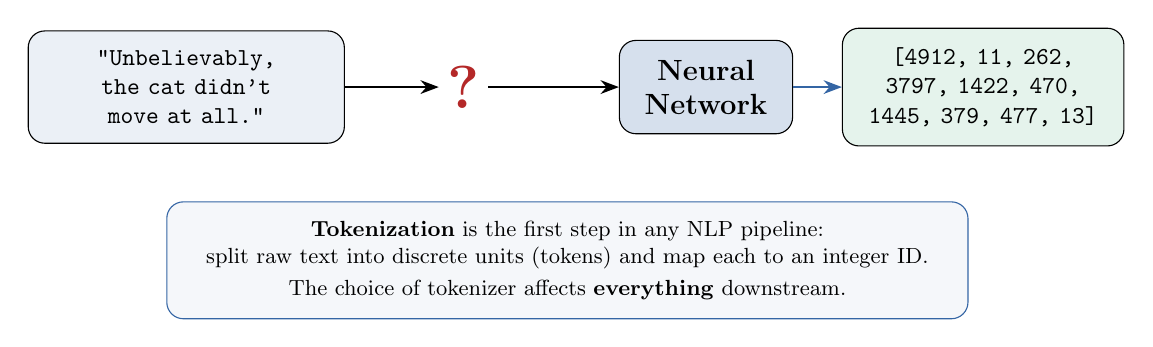
\begin{tikzpicture}[scale=0.88, transform shape,
  box/.style={draw, rounded corners=6pt, minimum height=1.2cm, align=center, font=\normalsize, inner sep=8pt}
]
  % Input text
  \node[box, fill=popblue!10, text width=4cm] (text) at (-5, 0) {
    \texttt{"Unbelievably,\\the cat didn't\\move at all."}
  };

  % Question mark
  \node[font=\Huge\bfseries, text=warnred] (q) at (-1, 0) {?};

  % Model
  \node[box, fill=popblue!20, minimum width=2.5cm, font=\large\bfseries] (model) at (2.5, 0) {Neural\\Network};

  % Numbers
  \node[box, fill=paramgreen!10, text width=3.5cm] (nums) at (6.5, 0) {
    \texttt{[4912, 11, 262,}\\
    \texttt{3797, 1422, 470,}\\
    \texttt{1445, 379, 477, 13]}
  };

  \draw[-{Stealth}, thick] (text) -- (q);
  \draw[-{Stealth}, thick] (q) -- (model);
  \draw[-{Stealth}, thick, popblue] (model) -- (nums);

  % Bottom annotation
  \node[draw=popblue, fill=popblue!5, rounded corners=6pt, text width=11cm, align=center, inner sep=8pt, font=\small] at (0.5, -2.5) {
    \textbf{Tokenization} is the first step in any NLP pipeline:\\
    split raw text into discrete units (tokens) and map each to an integer ID.\\[2pt]
    The choice of tokenizer affects \textbf{everything} downstream.
  };
\end{tikzpicture}
\end{center}
\end{frame}

% ============================================================
% THREE LEVELS
% ============================================================
\begin{frame}
\frametitle{Three levels of granularity}

\begin{center}
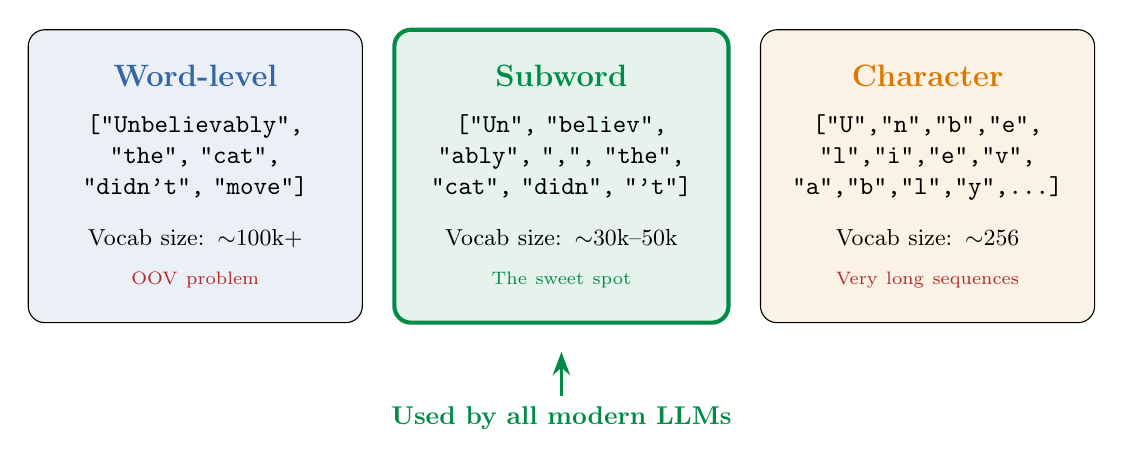
\begin{tikzpicture}[scale=0.93, transform shape,
  lvlbox/.style={draw, rounded corners=6pt, minimum width=4.3cm, minimum height=4cm, align=center, text width=4cm, inner sep=8pt}
]
  % Word-level
  \node[lvlbox, fill=popblue!10] (word) at (-5, 0) {
    \textbf{\large\textcolor{popblue}{Word-level}}\\[6pt]
    \texttt{["Unbelievably",}\\
    \texttt{"the", "cat",}\\
    \texttt{"didn't", "move"]}\\[8pt]
    {\small Vocab size: $\sim$100k+}\\[3pt]
    {\scriptsize\textcolor{warnred}{OOV problem}}
  };

  % Subword-level
  \node[lvlbox, fill=paramgreen!10, draw=paramgreen, line width=1.5pt] (sub) at (0, 0) {
    \textbf{\large\textcolor{paramgreen}{Subword}}\\[6pt]
    \texttt{["Un", "believ",}\\
    \texttt{"ably", ",", "the",}\\
    \texttt{"cat", "didn", "'t"]}\\[8pt]
    {\small Vocab size: $\sim$30k--50k}\\[3pt]
    {\scriptsize\textcolor{paramgreen}{The sweet spot}}
  };

  % Character-level
  \node[lvlbox, fill=orange1!10] (char) at (5, 0) {
    \textbf{\large\textcolor{orange1}{Character}}\\[6pt]
    \texttt{["U","n","b","e",}\\
    \texttt{"l","i","e","v",}\\
    \texttt{"a","b","l","y",...]}\\[8pt]
    {\small Vocab size: $\sim$256}\\[3pt]
    {\scriptsize\textcolor{warnred}{Very long sequences}}
  };

  % Arrow showing the sweet spot
  \draw[very thick, paramgreen, -{Stealth}] (0, -3) -- (0, -2.4);
  \node[font=\normalsize\bfseries, paramgreen] at (0, -3.3) {Used by all modern LLMs};
\end{tikzpicture}
\end{center}
\end{frame}

% ============================================================
% WORD-LEVEL: THE OOV PROBLEM
% ============================================================
\begin{frame}
\frametitle{Word-level tokenization and the OOV problem}
\vspace{-0.2cm}
\begin{center}
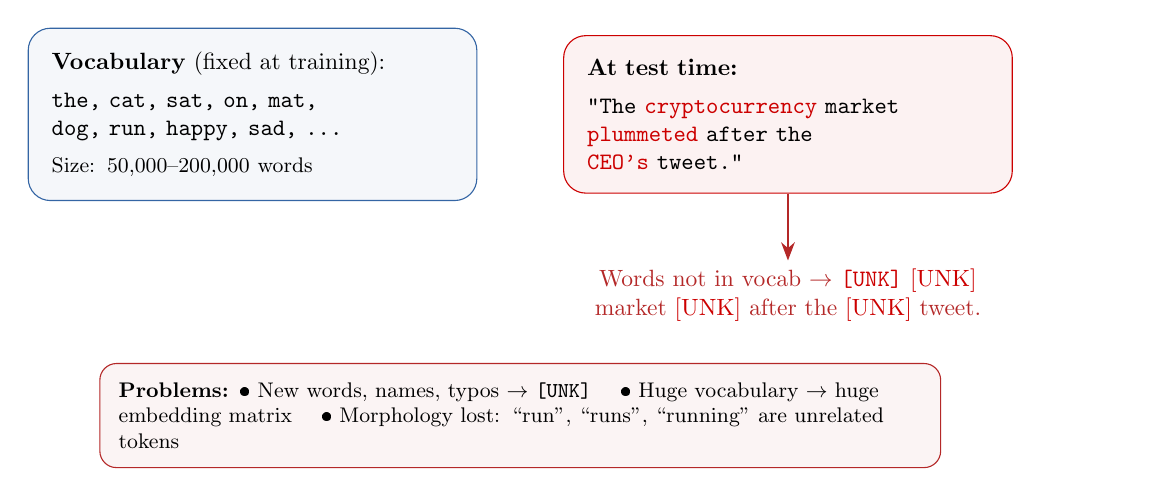
\begin{tikzpicture}[scale=0.85, transform shape]
  % Vocabulary box
  \node[draw=popblue, fill=popblue!5, rounded corners=8pt, text width=6cm, align=left, inner sep=10pt] (vocab) at (-4, 1) {
    \textbf{Vocabulary} (fixed at training):\\[4pt]
    \texttt{the, cat, sat, on, mat,}\\
    \texttt{dog, run, happy, sad, ...}\\[4pt]
    {\small Size: 50,000--200,000 words}
  };

  % Test-time input
  \node[draw=sampred, fill=sampred!5, rounded corners=8pt, text width=6cm, align=left, inner sep=10pt] (test) at (4, 1) {
    \textbf{At test time:}\\[4pt]
    \texttt{"The \textcolor{sampred}{cryptocurrency} market}\\
    \texttt{\textcolor{sampred}{plummeted} after the}\\
    \texttt{\textcolor{sampred}{CEO's} tweet."}
  };

  % Arrow
  \draw[-{Stealth}, thick, warnred] (test.south) -- ++(0, -1)
    node[below, text width=10cm, align=center, font=\normalsize] {
      Words not in vocab $\to$ \texttt{\textcolor{sampred}{[UNK]}} \textcolor{sampred}{[UNK]} market \textcolor{sampred}{[UNK]} after the \textcolor{sampred}{[UNK]} tweet.
    };

  % Problems list
  \node[draw=warnred, fill=warnred!5, rounded corners=6pt, text width=12cm, align=left, inner sep=8pt, font=\small] at (0, -3.5) {
    \textbf{Problems:}
    \textbullet\ New words, names, typos $\to$ \texttt{[UNK]} \quad
    \textbullet\ Huge vocabulary $\to$ huge embedding matrix \quad
    \textbullet\ Morphology lost: ``run'', ``runs'', ``running'' are unrelated tokens
  };
\end{tikzpicture}
\end{center}
\end{frame}

% ============================================================
% CHARACTER-LEVEL: TOO FINE
% ============================================================
\begin{frame}
\frametitle{Character-level: no unknowns, but\ldots}
\vspace{-0.4cm}
\begin{center}
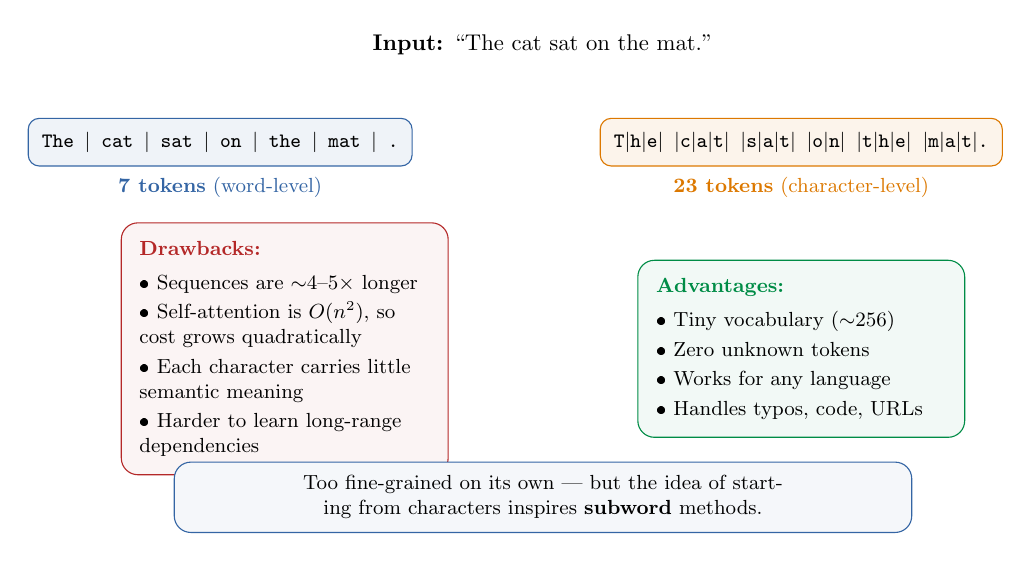
\begin{tikzpicture}[scale=0.82, transform shape]
  % The sentence
  \node[font=\normalsize] at (0, 3.5) {\textbf{Input:} ``The cat sat on the mat.''};

  % Word tokens
  \node[draw=popblue, fill=popblue!8, rounded corners=4pt, inner sep=6pt, font=\small] at (-5, 2) {
    \texttt{The \textbar{} cat \textbar{} sat \textbar{} on \textbar{} the \textbar{} mat \textbar{} .}
  };
  \node[font=\small, popblue] at (-5, 1.3) {\textbf{7 tokens} (word-level)};

  % Character tokens
  \node[draw=orange1, fill=orange1!8, rounded corners=4pt, inner sep=6pt, font=\small] at (4, 2) {
    \texttt{T\textbar h\textbar e\textbar{} \textbar c\textbar a\textbar t\textbar{} \textbar s\textbar a\textbar t\textbar{} \textbar o\textbar n\textbar{} \textbar t\textbar h\textbar e\textbar{} \textbar m\textbar a\textbar t\textbar .}
  };
  \node[font=\small, orange1] at (4, 1.3) {\textbf{23 tokens} (character-level)};

  % Problems
  \node[draw=warnred, fill=warnred!5, rounded corners=6pt, minimum width=5cm, minimum height=2.5cm, text width=4.5cm, align=left, inner sep=8pt, font=\small] at (-4, -1.2) {
    \textbf{\textcolor{warnred}{Drawbacks:}}\\[4pt]
    \textbullet\ Sequences are $\sim$4--5$\times$ longer\\[2pt]
    \textbullet\ Self-attention is $O(n^2)$, so cost grows quadratically\\[2pt]
    \textbullet\ Each character carries little semantic meaning\\[2pt]
    \textbullet\ Harder to learn long-range dependencies
  };

  % Advantages
  \node[draw=paramgreen, fill=paramgreen!5, rounded corners=6pt, minimum width=5cm, minimum height=2.5cm, text width=4.5cm, align=left, inner sep=8pt, font=\small] at (4, -1.2) {
    \textbf{\textcolor{paramgreen}{Advantages:}}\\[4pt]
    \textbullet\ Tiny vocabulary ($\sim$256)\\[2pt]
    \textbullet\ Zero unknown tokens\\[2pt]
    \textbullet\ Works for any language\\[2pt]
    \textbullet\ Handles typos, code, URLs
  };

  % Verdict
  \node[draw=popblue, fill=popblue!5, rounded corners=6pt, text width=11cm, align=center, inner sep=6pt, font=\small] at (0, -3.5) {
    Too fine-grained on its own --- but the idea of starting from characters inspires \textbf{subword} methods.
  };
\end{tikzpicture}
\end{center}
\end{frame}

% ============================================================
% SUBWORD: THE SWEET SPOT
% ============================================================
\begin{frame}
\frametitle{Subword tokenization: the key insight}
\vspace{-0.3cm}
\begin{center}
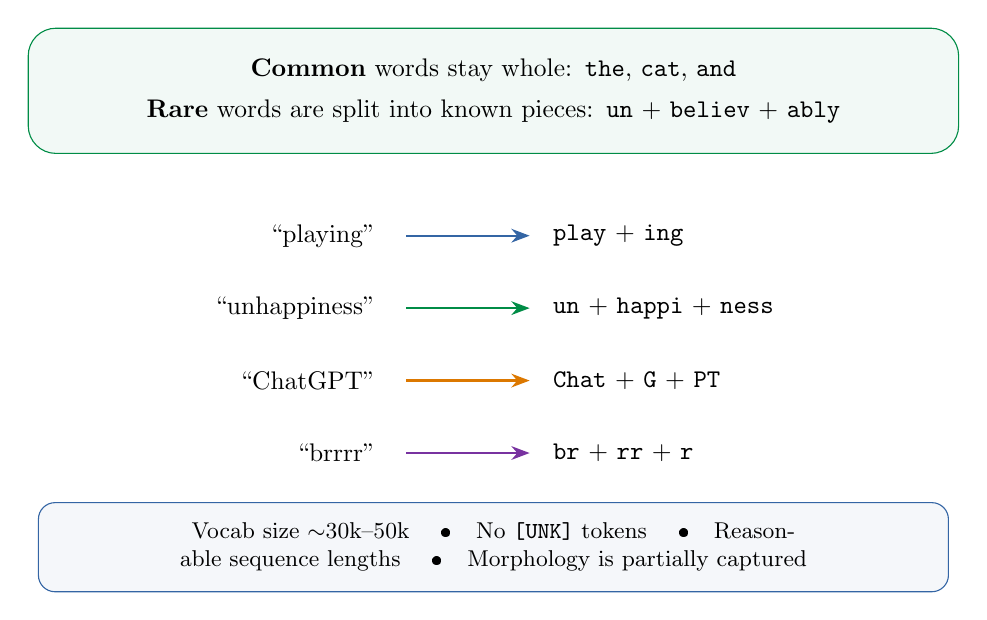
\begin{tikzpicture}[scale=0.92, transform shape]
  % The insight
  \node[draw=paramgreen, fill=paramgreen!5, rounded corners=10pt, text width=12cm, align=center, inner sep=12pt, font=\normalsize] at (0, 2.5) {
    \textbf{Common} words stay whole: \texttt{the}, \texttt{cat}, \texttt{and}\\[4pt]
    \textbf{Rare} words are split into known pieces: \texttt{un} + \texttt{believ} + \texttt{ably}
  };

  % Example decompositions
  \begin{scope}[yshift=-1cm]
    \node[font=\normalsize, anchor=east] at (-1.5, 1.5) {``playing''};
    \draw[-{Stealth}, thick, popblue] (-1.2, 1.5) -- (0.5, 1.5);
    \node[font=\normalsize, anchor=west] at (0.7, 1.5) {\texttt{play} + \texttt{ing}};

    \node[font=\normalsize, anchor=east] at (-1.5, 0.5) {``unhappiness''};
    \draw[-{Stealth}, thick, paramgreen] (-1.2, 0.5) -- (0.5, 0.5);
    \node[font=\normalsize, anchor=west] at (0.7, 0.5) {\texttt{un} + \texttt{happi} + \texttt{ness}};

    \node[font=\normalsize, anchor=east] at (-1.5, -0.5) {``ChatGPT''};
    \draw[-{Stealth}, thick, orange1] (-1.2, -0.5) -- (0.5, -0.5);
    \node[font=\normalsize, anchor=west] at (0.7, -0.5) {\texttt{Chat} + \texttt{G} + \texttt{PT}};

    \node[font=\normalsize, anchor=east] at (-1.5, -1.5) {``brrrr''};
    \draw[-{Stealth}, thick, violet1] (-1.2, -1.5) -- (0.5, -1.5);
    \node[font=\normalsize, anchor=west] at (0.7, -1.5) {\texttt{br} + \texttt{rr} + \texttt{r}};
  \end{scope}

  % Benefits summary
  \node[draw=popblue, fill=popblue!5, rounded corners=6pt, text width=12cm, align=center, inner sep=8pt, font=\small] at (0, -3.8) {
    Vocab size $\sim$30k--50k \quad\textbullet\quad
    No \texttt{[UNK]} tokens \quad\textbullet\quad
    Reasonable sequence lengths \quad\textbullet\quad
    Morphology is partially captured
  };
\end{tikzpicture}
\end{center}
\end{frame}

% ============================================================
% BPE: THE IDEA
% ============================================================
\begin{frame}
\frametitle{Byte-Pair Encoding (BPE): the idea}

\begin{center}
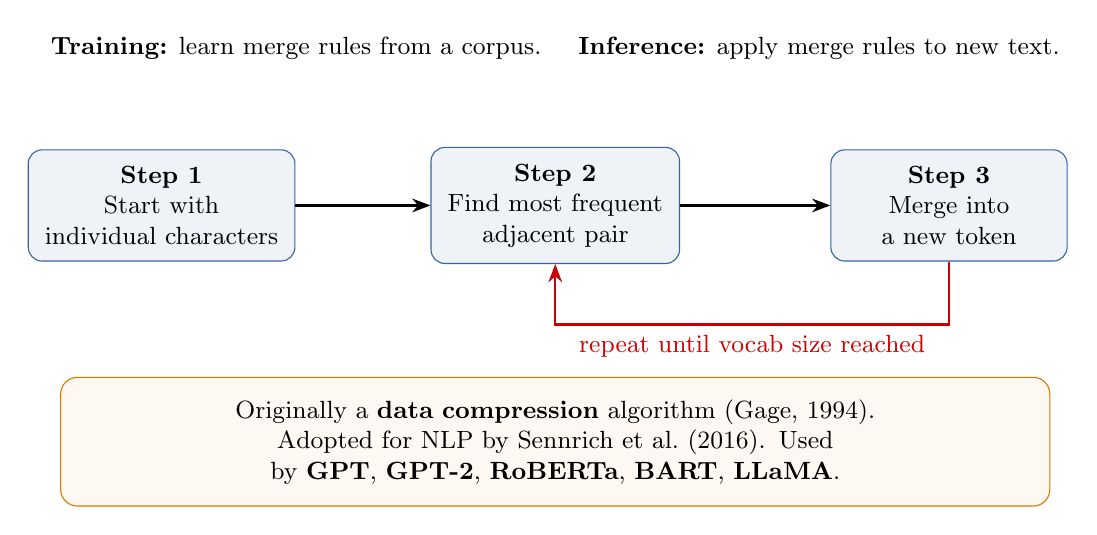
\begin{tikzpicture}[
  bpestep/.style={draw=popblue, fill=popblue!8, rounded corners=5pt, minimum width=3cm, minimum height=1cm, align=center, font=\small, inner sep=6pt}
]
  % Steps
  \node[bpestep] (s1) at (-5, 0) {\textbf{Step 1}\\Start with\\individual characters};
  \node[bpestep] (s2) at (0, 0) {\textbf{Step 2}\\Find most frequent\\adjacent pair};
  \node[bpestep] (s3) at (5, 0) {\textbf{Step 3}\\Merge into\\a new token};

  \draw[-{Stealth}, thick] (s1) -- (s2);
  \draw[-{Stealth}, thick] (s2) -- (s3);

  % Loop arrow
  \draw[-{Stealth}, thick, sampred] (s3.south) -- ++(0, -0.8) -| (s2.south)
    node[pos=0.25, below, font=\small] {repeat until vocab size reached};

  % Origin note
  \node[draw=orange1, fill=orange1!5, rounded corners=6pt, text width=12cm, align=center, inner sep=8pt, font=\small] at (0, -3) {
    Originally a \textbf{data compression} algorithm (Gage, 1994).\\
    Adopted for NLP by Sennrich et al.\ (2016). Used by \textbf{GPT}, \textbf{GPT-2}, \textbf{RoBERTa}, \textbf{BART}, \textbf{LLaMA}.
  };

  % Key properties
  \node[font=\small] at (0, 2) {
    \textbf{Training:} learn merge rules from a corpus.
    \quad\textbf{Inference:} apply merge rules to new text.
  };
\end{tikzpicture}
\end{center}
\end{frame}

% ============================================================
% BPE: WORKED EXAMPLE
% ============================================================
\begin{frame}
\frametitle{BPE: worked example}
\vspace{-0.3cm}
{\small\textbf{Corpus:} \texttt{hug} (10), \texttt{pug} (5), \texttt{pun} (12), \texttt{bun} (4), \texttt{hugs} (5)}

\vspace{0.1cm}
\begin{center}
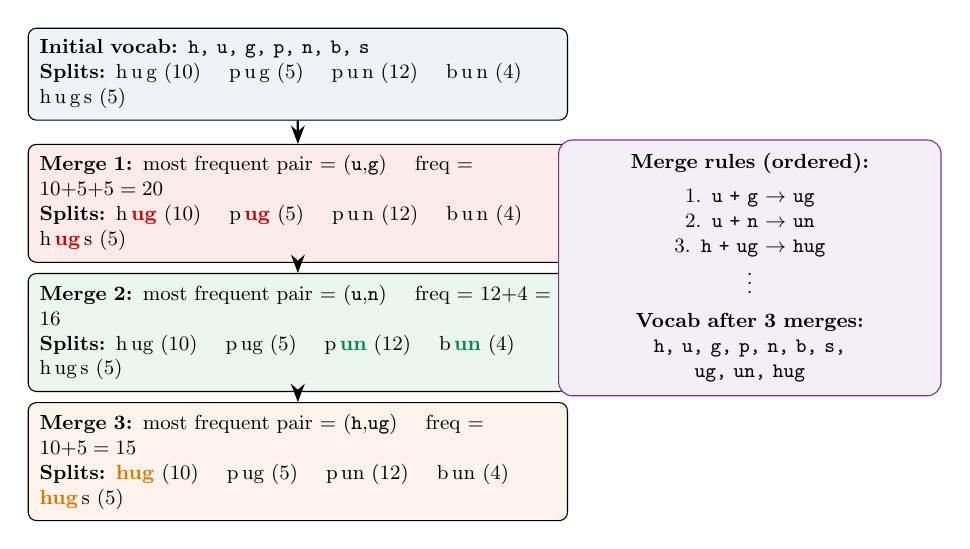
\begin{tikzpicture}[scale=0.82, transform shape]
  % Initial
  \node[draw, rounded corners=3pt, fill=popblue!8, inner sep=5pt, font=\small, text width=8cm, align=left] (init) at (0, 3.5) {
    \textbf{Initial vocab:} \texttt{h, u, g, p, n, b, s}\\
    \textbf{Splits:} h\,u\,g (10) \quad p\,u\,g (5) \quad p\,u\,n (12) \quad b\,u\,n (4) \quad h\,u\,g\,s (5)
  };

  % Merge 1
  \node[draw, rounded corners=3pt, fill=sampred!8, inner sep=5pt, font=\small, text width=8cm, align=left] (m1) at (0, 1.5) {
    \textbf{Merge 1:} most frequent pair = (\texttt{u},\texttt{g}) \quad freq = $10{+}5{+}5 = 20$\\
    \textbf{Splits:} h\,\textcolor{sampred}{\textbf{ug}} (10) \quad p\,\textcolor{sampred}{\textbf{ug}} (5) \quad p\,u\,n (12) \quad b\,u\,n (4) \quad h\,\textcolor{sampred}{\textbf{ug}}\,s (5)
  };

  % Merge 2
  \node[draw, rounded corners=3pt, fill=paramgreen!8, inner sep=5pt, font=\small, text width=8cm, align=left] (m2) at (0, -0.5) {
    \textbf{Merge 2:} most frequent pair = (\texttt{u},\texttt{n}) \quad freq = $12{+}4 = 16$\\
    \textbf{Splits:} h\,ug (10) \quad p\,ug (5) \quad p\,\textcolor{paramgreen}{\textbf{un}} (12) \quad b\,\textcolor{paramgreen}{\textbf{un}} (4) \quad h\,ug\,s (5)
  };

  % Merge 3
  \node[draw, rounded corners=3pt, fill=orange1!8, inner sep=5pt, font=\small, text width=8cm, align=left] (m3) at (0, -2.5) {
    \textbf{Merge 3:} most frequent pair = (\texttt{h},\texttt{ug}) \quad freq = $10{+}5 = 15$\\
    \textbf{Splits:} \textcolor{orange1}{\textbf{hug}} (10) \quad p\,ug (5) \quad p\,un (12) \quad b\,un (4) \quad \textcolor{orange1}{\textbf{hug}}\,s (5)
  };

  % Arrows
  \draw[-{Stealth}, thick] (init) -- (m1);
  \draw[-{Stealth}, thick] (m1) -- (m2);
  \draw[-{Stealth}, thick] (m2) -- (m3);

  % Final vocab
  \node[draw=violet1, fill=violet1!8, rounded corners=5pt, font=\small, text width=5.5cm, align=center, inner sep=6pt] at (7, 0.5) {
    \textbf{Merge rules (ordered):}\\[4pt]
    1. \texttt{u + g} $\to$ \texttt{ug}\\
    2. \texttt{u + n} $\to$ \texttt{un}\\
    3. \texttt{h + ug} $\to$ \texttt{hug}\\
    $\vdots$\\[4pt]
    \textbf{Vocab after 3 merges:}\\
    \texttt{h, u, g, p, n, b, s,}\\
    \texttt{ug, un, hug}
  };
\end{tikzpicture}
\end{center}
\end{frame}

% ============================================================
% BPE: INFERENCE
% ============================================================
\begin{frame}
\frametitle{BPE: tokenizing new text}
\vspace{-0.3cm}
\textbf{Given} the learned merge rules, tokenize a new word:

\vspace{0.1cm}
\begin{center}
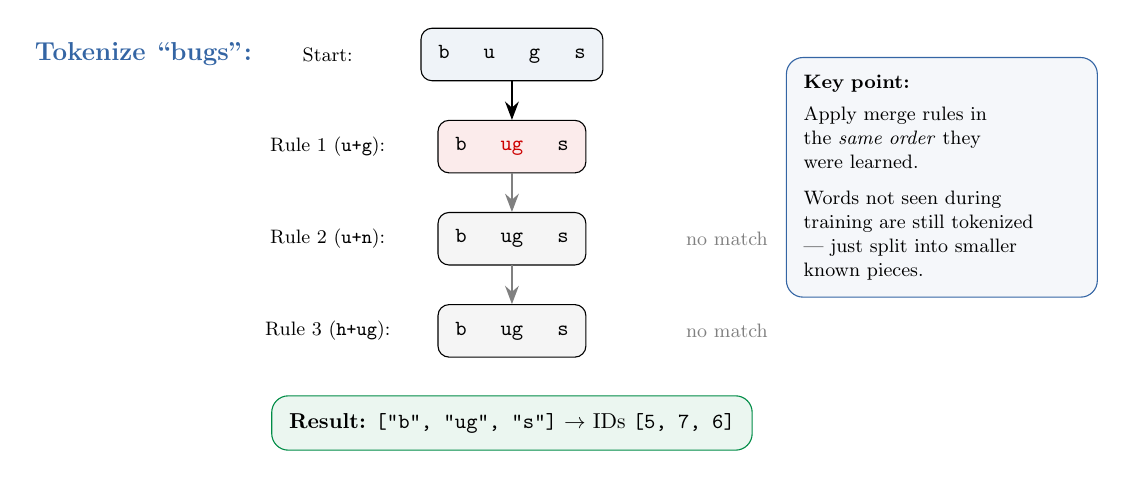
\begin{tikzpicture}[scale=0.78, transform shape]
  % Example word: "bugs"
  \node[font=\large\bfseries, popblue] at (-6, 2) {Tokenize ``bugs'':};

  % Step by step
  \node[draw, fill=popblue!8, rounded corners=4pt, font=\ttfamily\normalsize, inner sep=8pt] (s0) at (0, 2) {b \quad u \quad g \quad s};
  \node[font=\small] at (-3, 2) {Start:};

  \node[draw, fill=sampred!8, rounded corners=4pt, font=\ttfamily\normalsize, inner sep=8pt] (s1) at (0, 0.5) {b \quad \textcolor{sampred}{\textbf{ug}} \quad s};
  \node[font=\small] at (-3, 0.5) {Rule 1 (\texttt{u+g}):};

  \node[draw, fill=gray!8, rounded corners=4pt, font=\ttfamily\normalsize, inner sep=8pt] (s2) at (0, -1) {b \quad ug \quad s};
  \node[font=\small] at (-3, -1) {Rule 2 (\texttt{u+n}):};
  \node[font=\small, gray] at (3.5, -1) {no match};

  \node[draw, fill=gray!8, rounded corners=4pt, font=\ttfamily\normalsize, inner sep=8pt] (s3) at (0, -2.5) {b \quad ug \quad s};
  \node[font=\small] at (-3, -2.5) {Rule 3 (\texttt{h+ug}):};
  \node[font=\small, gray] at (3.5, -2.5) {no match};

  \draw[-{Stealth}, thick] (s0) -- (s1);
  \draw[-{Stealth}, thick, gray] (s1) -- (s2);
  \draw[-{Stealth}, thick, gray] (s2) -- (s3);

  % Result
  \node[draw=paramgreen, fill=paramgreen!8, rounded corners=6pt, font=\normalsize, inner sep=8pt] at (0, -4) {
    \textbf{Result:} \texttt{["b", "ug", "s"]} $\to$ IDs \texttt{[5, 7, 6]}
  };

  % Side note
  \node[draw=popblue, fill=popblue!5, rounded corners=6pt, text width=4.5cm, align=left, inner sep=8pt, font=\small] at (7, 0) {
    \textbf{Key point:}\\[4pt]
    Apply merge rules in\\
    the \textit{same order} they\\
    were learned.\\[6pt]
    Words not seen during\\
    training are still tokenized\\
    --- just split into smaller\\
    known pieces.
  };
\end{tikzpicture}
\end{center}
\end{frame}

% ============================================================
% BYTE-LEVEL BPE
% ============================================================
\begin{frame}
\frametitle{Byte-level BPE (GPT-2, GPT-3, LLaMA)}

\begin{center}
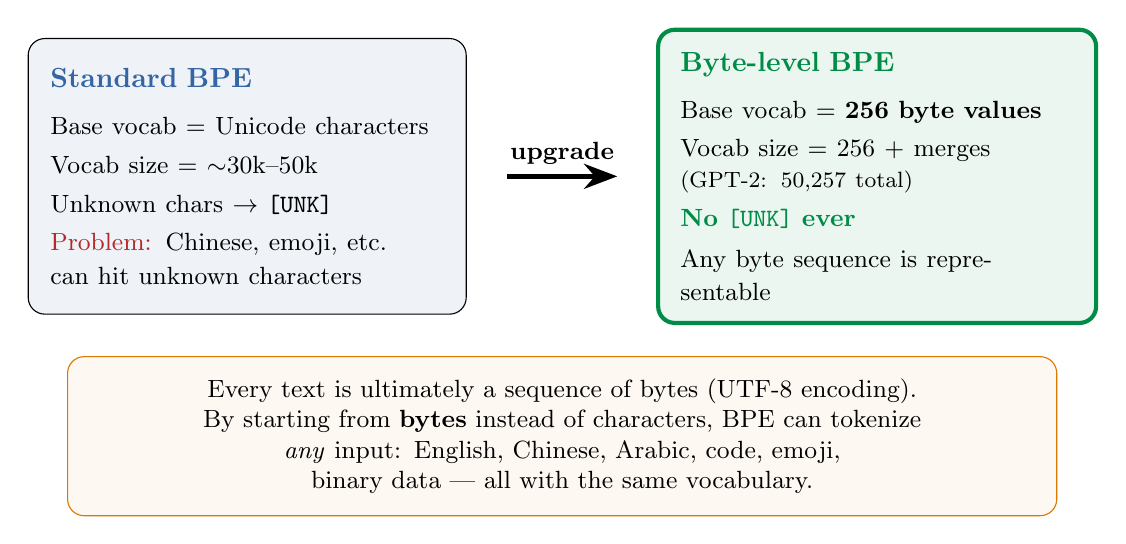
\begin{tikzpicture}[
  compbox/.style={draw, rounded corners=6pt, minimum width=5.5cm, minimum height=3.5cm, text width=5cm, align=left, inner sep=8pt}
]
  % Standard BPE
  \node[compbox, fill=popblue!8] at (-4, 0.5) {
    \textbf{\textcolor{popblue}{Standard BPE}}\\[6pt]
    \small
    Base vocab = Unicode characters\\[3pt]
    Vocab size = $\sim$30k--50k\\[3pt]
    Unknown chars $\to$ \texttt{[UNK]}\\[3pt]
    \textcolor{warnred}{Problem:} Chinese, emoji, etc.\\ can hit unknown characters
  };

  % Byte-level BPE
  \node[compbox, fill=paramgreen!8, draw=paramgreen, line width=1.5pt] at (4, 0.5) {
    \textbf{\textcolor{paramgreen}{Byte-level BPE}}\\[6pt]
    \small
    Base vocab = \textbf{256 byte values}\\[3pt]
    Vocab size = 256 + merges\\
    {\footnotesize (GPT-2: 50,257 total)}\\[3pt]
    \textcolor{paramgreen}{\textbf{No \texttt{[UNK]} ever}}\\[3pt]
    Any byte sequence is representable
  };

  % Arrow
  \draw[-{Stealth}, very thick, line width=2pt] (-0.7, 0.5) -- (0.7, 0.5)
    node[midway, above, font=\small\bfseries] {upgrade};

  % Explanation
  \node[draw=orange1, fill=orange1!5, rounded corners=6pt, text width=12cm, align=center, inner sep=8pt, font=\small] at (0, -2.8) {
    Every text is ultimately a sequence of bytes (UTF-8 encoding).\\
    By starting from \textbf{bytes} instead of characters, BPE can tokenize\\
    \textit{any} input: English, Chinese, Arabic, code, emoji, binary data --- all with the same vocabulary.
  };
\end{tikzpicture}
\end{center}
\end{frame}

% ============================================================
% WORDPIECE (BERT)
% ============================================================
\begin{frame}
\frametitle{WordPiece (BERT, DistilBERT)}

\begin{center}
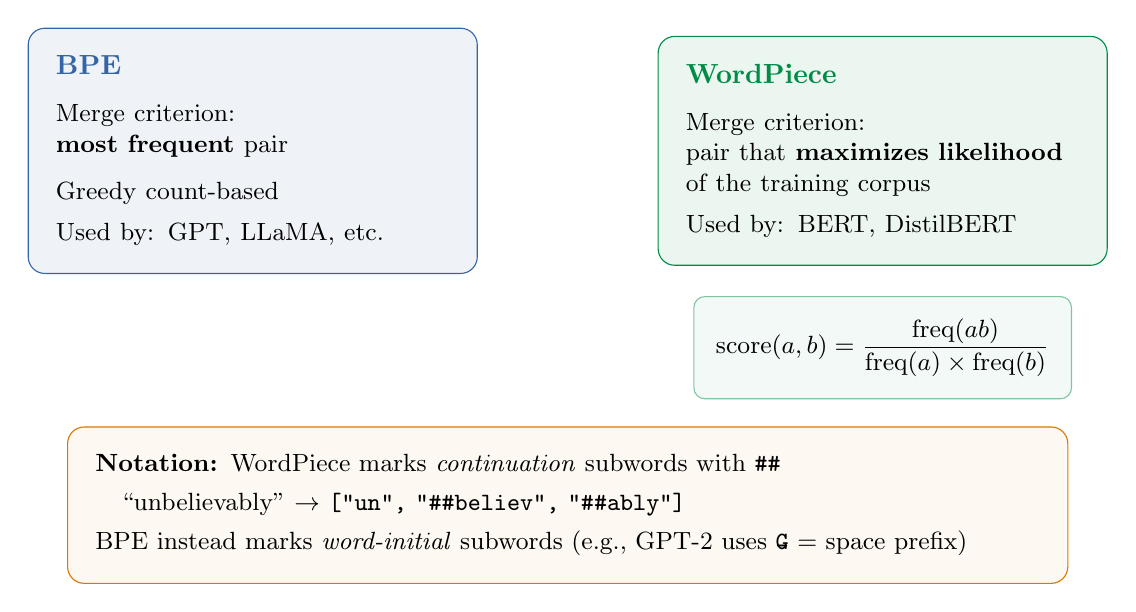
\begin{tikzpicture}
  % Comparison with BPE
  \node[draw=popblue, fill=popblue!8, rounded corners=6pt, minimum width=5.5cm, text width=5cm, align=left, inner sep=10pt] (bpe) at (-4, 1) {
    \textbf{\textcolor{popblue}{BPE}}\\[6pt]
    \small
    Merge criterion:\\
    \textbf{most frequent} pair\\[6pt]
    Greedy count-based\\[3pt]
    Used by: GPT, LLaMA, etc.
  };

  \node[draw=paramgreen, fill=paramgreen!8, rounded corners=6pt, minimum width=5.5cm, text width=5cm, align=left, inner sep=10pt] (wp) at (4, 1) {
    \textbf{\textcolor{paramgreen}{WordPiece}}\\[6pt]
    \small
    Merge criterion:\\
    pair that \textbf{maximizes likelihood}\\
    of the training corpus\\[3pt]
    Used by: BERT, DistilBERT
  };

  % Formula
  \node[draw=paramgreen!50, fill=paramgreen!5, rounded corners=4pt, font=\small, inner sep=8pt] at (4, -1.5) {
    $\displaystyle\text{score}(a, b) = \frac{\text{freq}(ab)}{\text{freq}(a) \times \text{freq}(b)}$
  };

  % Notation difference
  \node[draw=orange1, fill=orange1!5, rounded corners=6pt, text width=12cm, align=left, inner sep=10pt, font=\small] at (0, -3.5) {
    \textbf{Notation:} WordPiece marks \textit{continuation} subwords with \texttt{\#\#}\\[3pt]
    \quad ``unbelievably'' $\to$ \texttt{["un", "\#\#believ", "\#\#ably"]}\\[3pt]
    BPE instead marks \textit{word-initial} subwords (e.g., GPT-2 uses \texttt{\.{G}} = space prefix)
  };
\end{tikzpicture}
\end{center}
\end{frame}

% ============================================================
% UNIGRAM / SENTENCEPIECE
% ============================================================
\begin{frame}
\frametitle{Unigram LM and SentencePiece}

\begin{center}
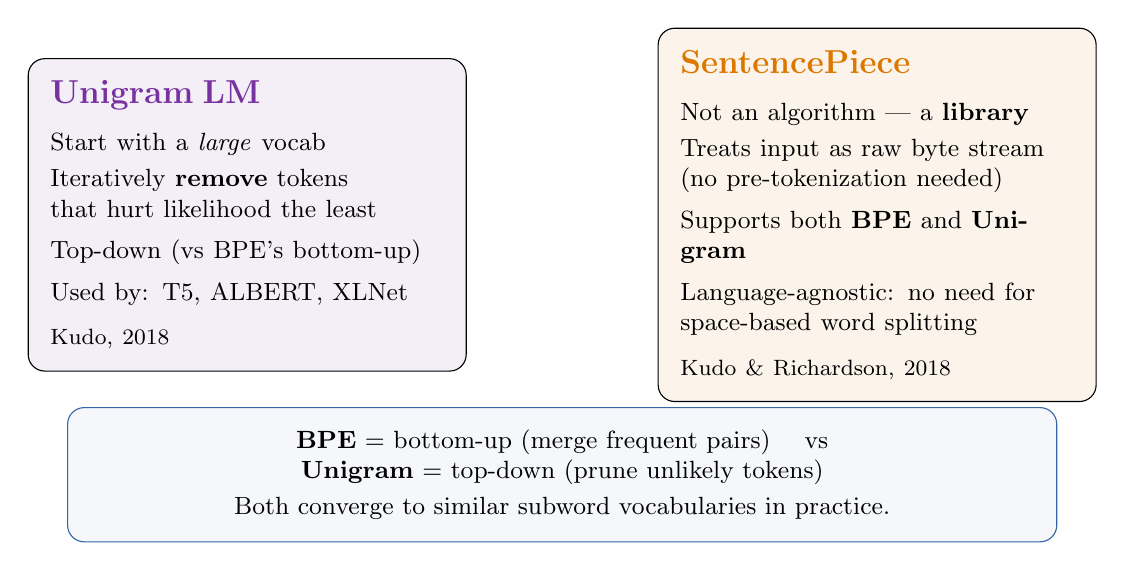
\begin{tikzpicture}[
  methbox/.style={draw, rounded corners=6pt, minimum width=5.5cm, minimum height=3.5cm, text width=5cm, align=left, inner sep=8pt}
]
  % Unigram
  \node[methbox, fill=violet1!8] at (-4, 0.5) {
    \textbf{\large\textcolor{violet1}{Unigram LM}}\\[6pt]
    \small
    Start with a \textit{large} vocab\\[2pt]
    Iteratively \textbf{remove} tokens\\
    that hurt likelihood the least\\[4pt]
    Top-down (vs BPE's bottom-up)\\[4pt]
    Used by: T5, ALBERT, XLNet\\[4pt]
    {\footnotesize Kudo, 2018}
  };

  % SentencePiece
  \node[methbox, fill=orange1!8] at (4, 0.5) {
    \textbf{\large\textcolor{orange1}{SentencePiece}}\\[6pt]
    \small
    Not an algorithm --- a \textbf{library}\\[2pt]
    Treats input as raw byte stream\\
    (no pre-tokenization needed)\\[4pt]
    Supports both \textbf{BPE} and \textbf{Unigram}\\[4pt]
    Language-agnostic: no need for\\
    space-based word splitting\\[4pt]
    {\footnotesize Kudo \& Richardson, 2018}
  };

  % Bottom comparison
  \node[draw=popblue, fill=popblue!5, rounded corners=6pt, text width=12cm, align=center, inner sep=8pt, font=\small] at (0, -2.8) {
    \textbf{BPE} = bottom-up (merge frequent pairs) \quad vs \quad
    \textbf{Unigram} = top-down (prune unlikely tokens)\\[2pt]
    Both converge to similar subword vocabularies in practice.
  };
\end{tikzpicture}
\end{center}
\end{frame}

% ============================================================
% WHY TOKENIZATION MATTERS
% ============================================================
\begin{frame}
\frametitle{Why tokenization matters: LLM quirks}
\vspace{-0.2cm}
\begin{center}
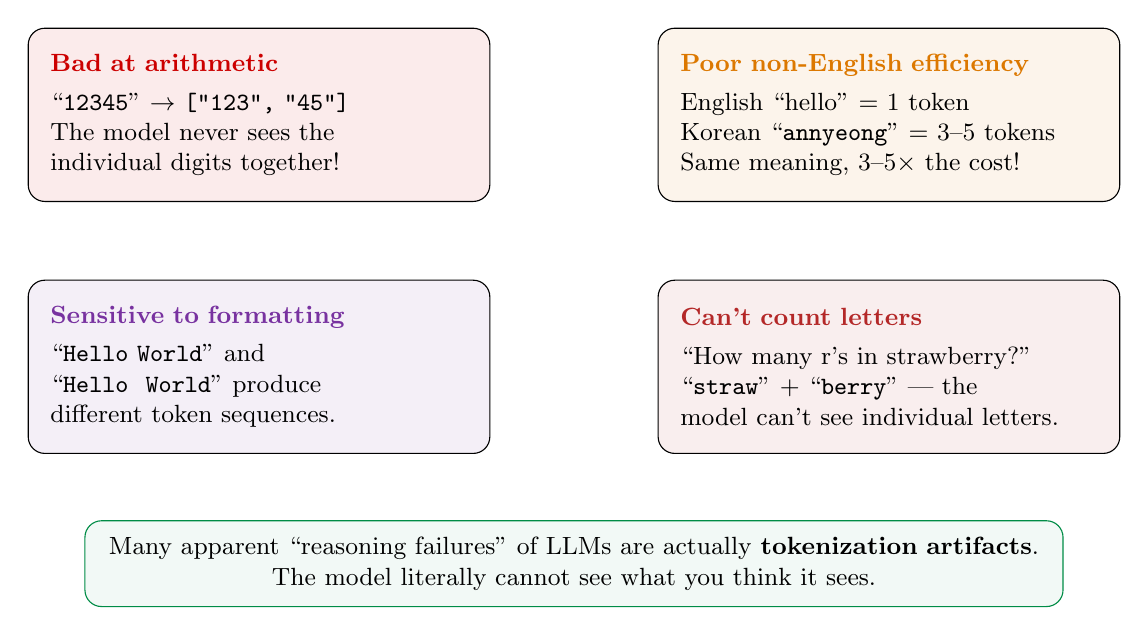
\begin{tikzpicture}[
  quirkbox/.style={draw, rounded corners=6pt, minimum width=5.8cm, minimum height=2.2cm, text width=5.3cm, align=left, inner sep=8pt, font=\small}
]
  % Quirk 1: Arithmetic
  \node[quirkbox, fill=sampred!8] at (-4, 2) {
    \textbf{\textcolor{sampred}{Bad at arithmetic}}\\[3pt]
    ``\texttt{12345}'' $\to$ \texttt{["123", "45"]}\\
    The model never sees the\\
    individual digits together!
  };

  % Quirk 2: Non-English
  \node[quirkbox, fill=orange1!8] at (4, 2) {
    \textbf{\textcolor{orange1}{Poor non-English efficiency}}\\[3pt]
    English ``hello'' = 1 token\\
    Korean ``$\text{\texttt{annyeong}}$'' = 3--5 tokens\\
    Same meaning, 3--5$\times$ the cost!
  };

  % Quirk 3: Trailing spaces
  \node[quirkbox, fill=violet1!8] at (-4, -1.2) {
    \textbf{\textcolor{violet1}{Sensitive to formatting}}\\[3pt]
    ``\texttt{Hello World}'' and\\
    ``\texttt{Hello{\ }{\ }World}'' produce\\
    different token sequences.
  };

  % Quirk 4: Can't count letters
  \node[quirkbox, fill=warnred!8] at (4, -1.2) {
    \textbf{\textcolor{warnred}{Can't count letters}}\\[3pt]
    ``How many r's in strawberry?''\\
    ``\texttt{straw}'' + ``\texttt{berry}'' --- the\\
    model can't see individual letters.
  };

  % Bottom note
  \node[draw=paramgreen, fill=paramgreen!5, rounded corners=6pt, text width=12cm, align=center, inner sep=6pt, font=\small] at (0, -3.7) {
    Many apparent ``reasoning failures'' of LLMs are actually \textbf{tokenization artifacts}.\\
    The model literally cannot see what you think it sees.
  };
\end{tikzpicture}
\end{center}
\end{frame}

% ============================================================
% VISUALIZING TOKENIZATION
% ============================================================
\begin{frame}
\frametitle{Visualizing: the same sentence, different tokenizers}
\vspace{-0.2cm}
{\small\textbf{Input:} ``The cat sat on the unbelievably soft mat''}

\vspace{0.2cm}
\begin{center}
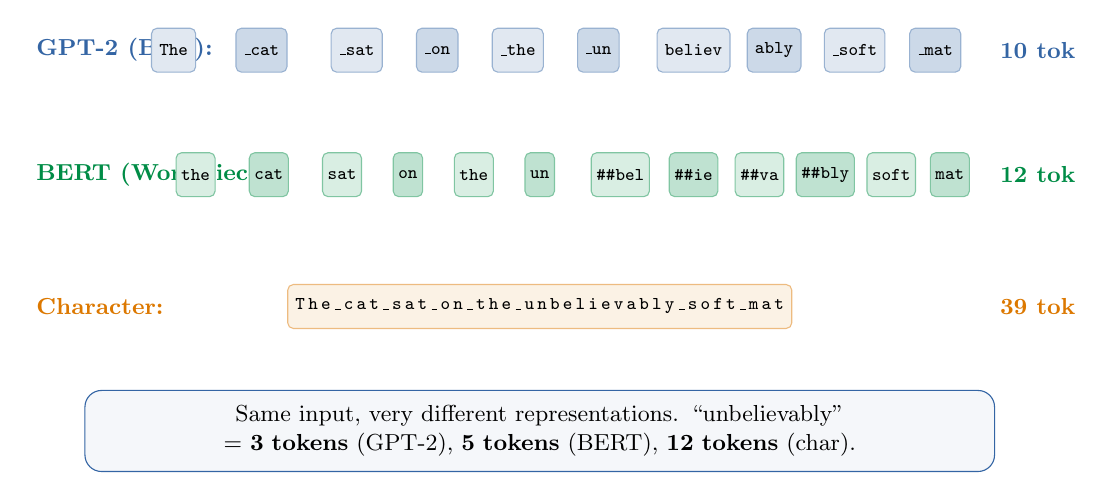
\begin{tikzpicture}[scale=0.93, transform shape]
  % GPT-2 tokenization
  \node[font=\small\bfseries, popblue, anchor=west] at (-7, 2) {GPT-2 (BPE):};
  \node[draw=popblue!50, fill=popblue!15, rounded corners=2pt, inner sep=3pt, font=\scriptsize\ttfamily, minimum height=0.6cm] at (-5, 2) {The};
  \node[draw=popblue!50, fill=popblue!25, rounded corners=2pt, inner sep=3pt, font=\scriptsize\ttfamily, minimum height=0.6cm] at (-3.8, 2) {\_cat};
  \node[draw=popblue!50, fill=popblue!15, rounded corners=2pt, inner sep=3pt, font=\scriptsize\ttfamily, minimum height=0.6cm] at (-2.5, 2) {\_sat};
  \node[draw=popblue!50, fill=popblue!25, rounded corners=2pt, inner sep=3pt, font=\scriptsize\ttfamily, minimum height=0.6cm] at (-1.4, 2) {\_on};
  \node[draw=popblue!50, fill=popblue!15, rounded corners=2pt, inner sep=3pt, font=\scriptsize\ttfamily, minimum height=0.6cm] at (-0.3, 2) {\_the};
  \node[draw=popblue!50, fill=popblue!25, rounded corners=2pt, inner sep=3pt, font=\scriptsize\ttfamily, minimum height=0.6cm] at (0.8, 2) {\_un};
  \node[draw=popblue!50, fill=popblue!15, rounded corners=2pt, inner sep=3pt, font=\scriptsize\ttfamily, minimum height=0.6cm] at (2.1, 2) {believ};
  \node[draw=popblue!50, fill=popblue!25, rounded corners=2pt, inner sep=3pt, font=\scriptsize\ttfamily, minimum height=0.6cm] at (3.2, 2) {ably};
  \node[draw=popblue!50, fill=popblue!15, rounded corners=2pt, inner sep=3pt, font=\scriptsize\ttfamily, minimum height=0.6cm] at (4.3, 2) {\_soft};
  \node[draw=popblue!50, fill=popblue!25, rounded corners=2pt, inner sep=3pt, font=\scriptsize\ttfamily, minimum height=0.6cm] at (5.4, 2) {\_mat};
  \node[font=\small\bfseries, popblue] at (6.8, 2) {10 tok};

  % BERT tokenization
  \node[font=\small\bfseries, paramgreen, anchor=west] at (-7, 0.3) {BERT (WordPiece):};
  \node[draw=paramgreen!50, fill=paramgreen!15, rounded corners=2pt, inner sep=2pt, font=\scriptsize\ttfamily, minimum height=0.6cm] at (-4.7, 0.3) {the};
  \node[draw=paramgreen!50, fill=paramgreen!25, rounded corners=2pt, inner sep=2pt, font=\scriptsize\ttfamily, minimum height=0.6cm] at (-3.7, 0.3) {cat};
  \node[draw=paramgreen!50, fill=paramgreen!15, rounded corners=2pt, inner sep=2pt, font=\scriptsize\ttfamily, minimum height=0.6cm] at (-2.7, 0.3) {sat};
  \node[draw=paramgreen!50, fill=paramgreen!25, rounded corners=2pt, inner sep=2pt, font=\scriptsize\ttfamily, minimum height=0.6cm] at (-1.8, 0.3) {on};
  \node[draw=paramgreen!50, fill=paramgreen!15, rounded corners=2pt, inner sep=2pt, font=\scriptsize\ttfamily, minimum height=0.6cm] at (-0.9, 0.3) {the};
  \node[draw=paramgreen!50, fill=paramgreen!25, rounded corners=2pt, inner sep=2pt, font=\scriptsize\ttfamily, minimum height=0.6cm] at (0, 0.3) {un};
  \node[draw=paramgreen!50, fill=paramgreen!15, rounded corners=2pt, inner sep=2pt, font=\scriptsize\ttfamily, minimum height=0.6cm] at (1.1, 0.3) {\#\#bel};
  \node[draw=paramgreen!50, fill=paramgreen!25, rounded corners=2pt, inner sep=2pt, font=\scriptsize\ttfamily, minimum height=0.6cm] at (2.1, 0.3) {\#\#ie};
  \node[draw=paramgreen!50, fill=paramgreen!15, rounded corners=2pt, inner sep=2pt, font=\scriptsize\ttfamily, minimum height=0.6cm] at (3, 0.3) {\#\#va};
  \node[draw=paramgreen!50, fill=paramgreen!25, rounded corners=2pt, inner sep=2pt, font=\scriptsize\ttfamily, minimum height=0.6cm] at (3.9, 0.3) {\#\#bly};
  \node[draw=paramgreen!50, fill=paramgreen!15, rounded corners=2pt, inner sep=2pt, font=\scriptsize\ttfamily, minimum height=0.6cm] at (4.8, 0.3) {soft};
  \node[draw=paramgreen!50, fill=paramgreen!25, rounded corners=2pt, inner sep=2pt, font=\scriptsize\ttfamily, minimum height=0.6cm] at (5.6, 0.3) {mat};
  \node[font=\small\bfseries, paramgreen] at (6.8, 0.3) {12 tok};

  % Character
  \node[font=\small\bfseries, orange1, anchor=west] at (-7, -1.5) {Character:};
  \node[draw=orange1!50, fill=orange1!10, rounded corners=2pt, inner sep=3pt, font=\scriptsize\ttfamily, minimum height=0.6cm] at (0, -1.5) {
    T\,h\,e\,\_\,c\,a\,t\,\_\,s\,a\,t\,\_\,o\,n\,\_\,t\,h\,e\,\_\,u\,n\,b\,e\,l\,i\,e\,v\,a\,b\,l\,y\,\_\,s\,o\,f\,t\,\_\,m\,a\,t
  };
  \node[font=\small\bfseries, orange1] at (6.8, -1.5) {39 tok};

  % Observation
  \node[draw=popblue, fill=popblue!5, rounded corners=6pt, text width=12cm, align=center, inner sep=6pt, font=\small] at (0, -3.2) {
    Same input, very different representations.
    ``unbelievably'' = \textbf{3 tokens} (GPT-2), \textbf{5 tokens} (BERT), \textbf{12 tokens} (char).
  };
\end{tikzpicture}
\end{center}
\end{frame}

% ============================================================
% SPECIAL TOKENS
% ============================================================
\begin{frame}
\frametitle{Special tokens}

\begin{center}
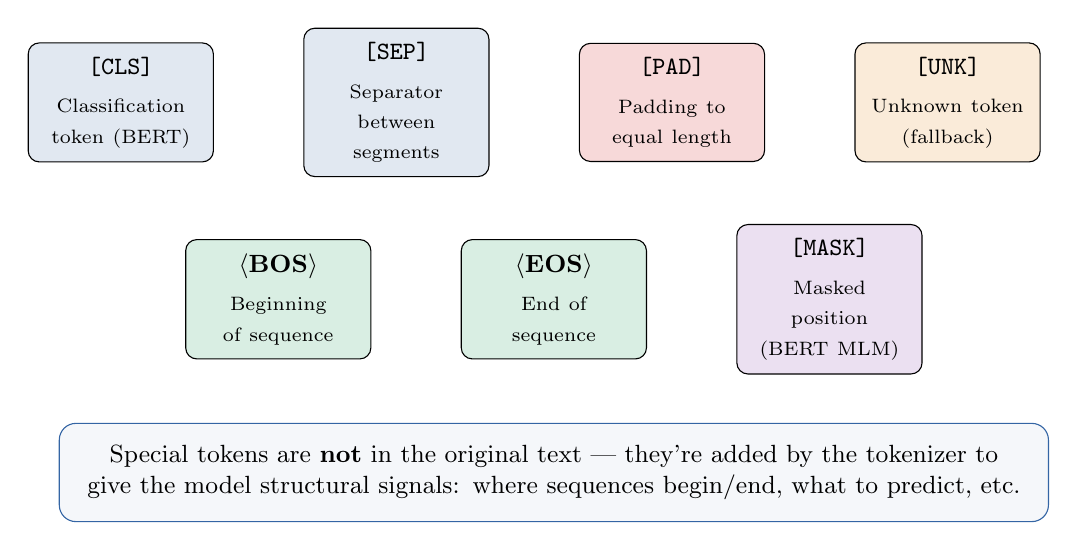
\begin{tikzpicture}[
  tokbox/.style={draw, rounded corners=4pt, minimum width=2.2cm, minimum height=1.5cm, align=center, font=\small, inner sep=5pt, text width=2cm}
]
  % Tokens
  \node[tokbox, fill=popblue!15] (cls) at (-5.5, 1.5) {
    \texttt{\textbf{[CLS]}}\\[3pt]
    {\scriptsize Classification token (BERT)}
  };
  \node[tokbox, fill=popblue!15] (sep) at (-2, 1.5) {
    \texttt{\textbf{[SEP]}}\\[3pt]
    {\scriptsize Separator between segments}
  };
  \node[tokbox, fill=sampred!15] (pad) at (1.5, 1.5) {
    \texttt{\textbf{[PAD]}}\\[3pt]
    {\scriptsize Padding to equal length}
  };
  \node[tokbox, fill=orange1!15] (unk) at (5, 1.5) {
    \texttt{\textbf{[UNK]}}\\[3pt]
    {\scriptsize Unknown token (fallback)}
  };

  \node[tokbox, fill=paramgreen!15] (bos) at (-3.5, -1) {
    \textbf{$\langle$BOS$\rangle$}\\[3pt]
    {\scriptsize Beginning of sequence}
  };
  \node[tokbox, fill=paramgreen!15] (eos) at (0, -1) {
    \textbf{$\langle$EOS$\rangle$}\\[3pt]
    {\scriptsize End of sequence}
  };
  \node[tokbox, fill=violet1!15] (mask) at (3.5, -1) {
    \texttt{\textbf{[MASK]}}\\[3pt]
    {\scriptsize Masked position (BERT MLM)}
  };

  % Annotation
  \node[draw=popblue, fill=popblue!5, rounded corners=6pt, text width=12cm, align=center, inner sep=8pt, font=\small] at (0, -3.2) {
    Special tokens are \textbf{not} in the original text --- they're added by the tokenizer
    to give the model structural signals: where sequences begin/end, what to predict, etc.
  };
\end{tikzpicture}
\end{center}
\end{frame}

% ============================================================
% COMPARISON TABLE
% ============================================================
\begin{frame}
\frametitle{Comparison of tokenization methods}

\vspace{-0.3cm}
\renewcommand{\arraystretch}{1.5}
\begin{center}
{\small
\begin{tabular}{>{\bfseries}l c c c c}
  \textbf{Method} & \textbf{Direction} & \textbf{Criterion} & \textbf{Vocab size} & \textbf{Used by} \\
  \hline
  \textcolor{popblue}{BPE} & Bottom-up & Frequency & 30k--50k & GPT, LLaMA \\[2pt]
  \textcolor{paramgreen}{WordPiece} & Bottom-up & Likelihood & 30k & BERT \\[2pt]
  \textcolor{violet1}{Unigram} & Top-down & Likelihood & 30k--50k & T5, XLNet \\[2pt]
  \textcolor{orange1}{Byte BPE} & Bottom-up & Frequency & 50k--100k & GPT-2/3/4 \\[2pt]
  \textcolor{sampred}{Character} & --- & --- & 256 & ByT5 \\
  \hline
\end{tabular}
}
\end{center}

\vspace{0.4cm}
\begin{center}
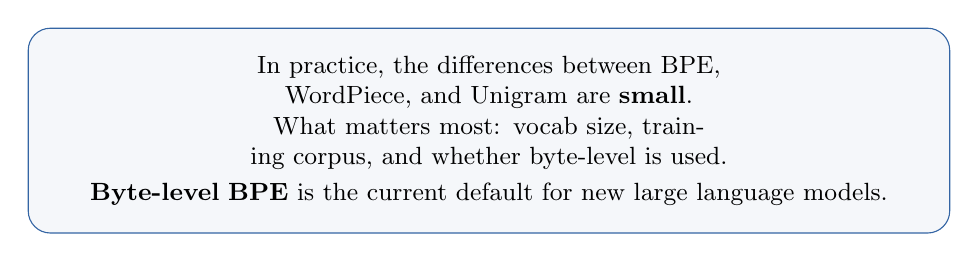
\begin{tikzpicture}
  \node[draw=popblue, fill=popblue!5, rounded corners=8pt, text width=11cm, align=center, inner sep=10pt, font=\small] {
    In practice, the differences between BPE, WordPiece, and Unigram are \textbf{small}.\\
    What matters most: vocab size, training corpus, and whether byte-level is used.\\[2pt]
    \textbf{Byte-level BPE} is the current default for new large language models.
  };
\end{tikzpicture}
\end{center}
\end{frame}

% ============================================================
% PRACTICAL: TRYING IT OUT
% ============================================================
\begin{frame}
\frametitle{Practical: tokenizers in action}

\begin{center}
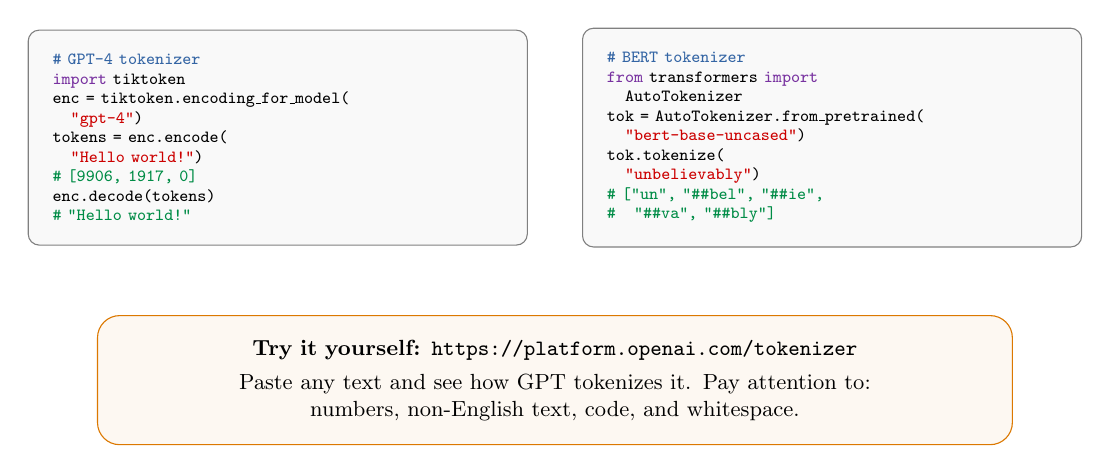
\begin{tikzpicture}[scale=0.88, transform shape]
  % Code box 1: tiktoken (GPT)
  \node[draw=gray, fill=gray!5, rounded corners=4pt, text width=6.5cm, align=left, inner sep=10pt, font=\ttfamily\scriptsize] at (-4, 1.2) {
    \textcolor{popblue}{\# GPT-4 tokenizer}\\
    \textcolor{violet1}{import} tiktoken\\
    enc = tiktoken.encoding\_for\_model(\\
    \quad \textcolor{sampred}{"gpt-4"})\\
    tokens = enc.encode(\\
    \quad \textcolor{sampred}{"Hello world!"})\\
    \textcolor{paramgreen}{\# [9906, 1917, 0]}\\
    enc.decode(tokens)\\
    \textcolor{paramgreen}{\# "Hello world!"}
  };

  % Code box 2: HuggingFace (BERT)
  \node[draw=gray, fill=gray!5, rounded corners=4pt, text width=6.5cm, align=left, inner sep=10pt, font=\ttfamily\scriptsize] at (4, 1.2) {
    \textcolor{popblue}{\# BERT tokenizer}\\
    \textcolor{violet1}{from} transformers \textcolor{violet1}{import}\\
    \quad AutoTokenizer\\
    tok = AutoTokenizer.from\_pretrained(\\
    \quad \textcolor{sampred}{"bert-base-uncased"})\\
    tok.tokenize(\\
    \quad \textcolor{sampred}{"unbelievably"})\\
    \textcolor{paramgreen}{\# ["un", "\#\#bel", "\#\#ie",}\\
    \textcolor{paramgreen}{\#\quad "\#\#va", "\#\#bly"]}
  };

  % Try it yourself
  \node[draw=orange1, fill=orange1!5, rounded corners=8pt, text width=12.5cm, align=center, inner sep=10pt, font=\small] at (0, -2.3) {
    \textbf{Try it yourself:} \texttt{https://platform.openai.com/tokenizer}\\[3pt]
    Paste any text and see how GPT tokenizes it. Pay attention to:\\
    numbers, non-English text, code, and whitespace.
  };
\end{tikzpicture}
\end{center}
\end{frame}

% ============================================================
% FURTHER READING
% ============================================================
\begin{frame}
\frametitle{Further reading}
\vspace{-0.3cm}
\begin{center}
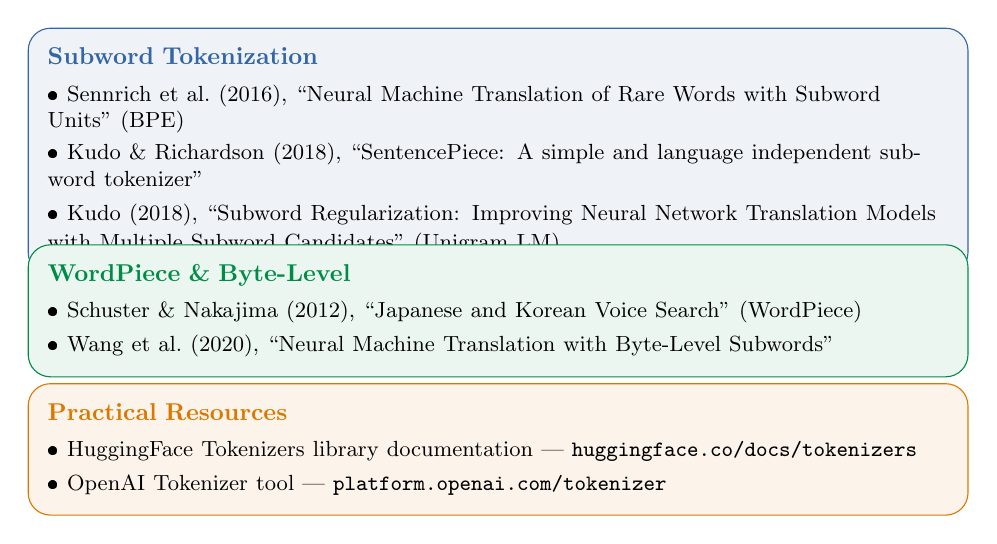
\begin{tikzpicture}[scale=0.88, transform shape]
  \node[draw=popblue, fill=popblue!8, rounded corners=8pt, text width=13cm, align=left, inner sep=8pt] at (0, 2.5) {
    \textbf{\textcolor{popblue}{Subword Tokenization}}\\[4pt]
    {\small
    \textbullet~Sennrich et al.\ (2016), ``Neural Machine Translation of Rare Words with Subword Units'' (BPE)\\[2pt]
    \textbullet~Kudo \& Richardson (2018), ``SentencePiece: A simple and language independent subword tokenizer''\\[2pt]
    \textbullet~Kudo (2018), ``Subword Regularization: Improving Neural Network Translation Models with Multiple Subword Candidates'' (Unigram LM)
    }
  };
  \node[draw=paramgreen, fill=paramgreen!8, rounded corners=8pt, text width=13cm, align=left, inner sep=8pt] at (0, 0.2) {
    \textbf{\textcolor{paramgreen}{WordPiece \& Byte-Level}}\\[4pt]
    {\small
    \textbullet~Schuster \& Nakajima (2012), ``Japanese and Korean Voice Search'' (WordPiece)\\[2pt]
    \textbullet~Wang et al.\ (2020), ``Neural Machine Translation with Byte-Level Subwords''
    }
  };
  \node[draw=orange1, fill=orange1!8, rounded corners=8pt, text width=13cm, align=left, inner sep=8pt] at (0, -1.8) {
    \textbf{\textcolor{orange1}{Practical Resources}}\\[4pt]
    {\small
    \textbullet~HuggingFace Tokenizers library documentation --- \texttt{huggingface.co/docs/tokenizers}\\[2pt]
    \textbullet~OpenAI Tokenizer tool --- \texttt{platform.openai.com/tokenizer}
    }
  };
\end{tikzpicture}
\end{center}
\end{frame}

% ============================================================
% QUESTIONS
% ============================================================
\begin{frame}
\begin{center}
  {\Huge\bfseries\textcolor{popblue}{Questions?}}

  \vspace{1cm}

  {\large Next: Evaluation --- Perplexity, BLEU, ROUGE}
\end{center}
\end{frame}

\end{document}
